\chapter{IMPLEMENTASI}
Tahap implementasi pada penelitian ini menggunakan memiliki beberapa tahap yang terbagi menjadi empat yaitu \textit{data collection}, \textit{data labelling}, \textit{training}, \textit{testing}.
Data collection pada penelitian ini adalah proses pengumpulan dataset yang dilakukan dengan melakukan akuisisi citra menggunakan webcam dan pengunduhan dataset \textit{public}. Data yang di dapatkan dari proses akuisisi citra akan dilakukan \textit{preprocessing} terlebih dahulu sebelum dilakukan proses labelling sesuai dengan klasifikasi. Tahap \textit{training} digunakan untuk ekstraksi fitur dataset yang disimpan dalam sebuah model. Model yang terbentuk akan dilakukan proses pengujian pada tahap testing.

\section{Data Collection}
Data yang digunakan dalam penelitian ini adalah data yang diampbil dari proses akuisisi citra dan dataset \textit{American Sign Language} dari \textit{Massey University}. Dataset yang diambil dari proses akuisisi citra sebanyak 1000 citra tangan yang diambil dari 10 orang. Selanjutnya untuk dataset \textit{American Sign Language} akan dilakukan preprocessing terlebih dahulu sebelum dijadikan format csv yang berisi nama dan lokasi citra.

\subsection{Implementasi Proses Akuisisi Citra}
Tahap akuisisi citra dilakukan bertujuan mendapatkan dataset untuk deteksi objek tangan sehingga dataset yang diambil adalah pose tangan dari subjek. Setiap subjek akan diambil sebanyak 100 citra sehingga menghasilkan 1000 citra. Pada program yang dibuat akan melakukan penyimpanan citra pada folder tertentu dengan setiap nama masing masing subjek. Gambar 5.1 menunjukan kode implementasi saat proses akuisisi citra berlangsung.
\begin{figure}[H]
	\centering
	\lstinputlisting[language=python]{collect-data-object-detection.py}
	\caption{Source code akuisisi citra}
\end{figure}

\subsection{Implementasi Data Augmentasi}
Proses augmentasi data digunakan untuk menduplikat citra dengan variasi yang berbeda. Pada proses augmentasi ini diterapkan untuk dataset \textit{American Sign Language} karena hanya memiliki 700 citra untuk 10 klasifikasi. Sebelum dilakukan augmentasi, citra pada dataset \textit{American Sign Language} akan dilakukan \textit{resize} pada ukuran (224x224). Augmentasi yang dilakukan berupa variasi intensitas cahaya, intensitas warna, operasi morfologi, \textit{filtering} dan rotasi.
\begin{figure}[H]
	\centering
	\lstinputlisting[language=python]{augmen.py}
	\caption{Source Code Augmentasi Citra}
\end{figure}
\subsection{Pembuatan file CSV}
Dataset dari pengenalan gestur akan dibuat file CSV yang berisi label dan lokasi dari setiap citra dalam dataset. Fungsi tocsv berikut adalah implementasi dari pembuatan file CSV
\begin{figure}[H]
	\centering
	\lstinputlisting[language=python]{csv.py}
	\caption{Source Code Pembuatan file CSV}
\end{figure}
Hasil dari implementasi csv tersebut akan digunakan untuk refrensi input dalam proses pelatihan pengenalan gestur. Berikut adalah hasil dari pembuatan file csv dataset.
% TODO: \usepackage{graphicx} required
\begin{figure}[H]
	\centering
	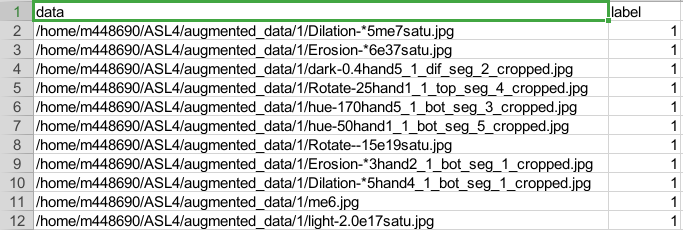
\includegraphics[width=0.7\linewidth]{csv}
	\caption{hasil file csv}
	\label{fig:csv}
\end{figure}
\section{Implementasi Data Labelling}
Pelabelan sebuah citra dilakukan untuk memberikan pengenalan suatu objek yang ada dalam sebuah citra, pada proses pelabelan menyimpan anotasi yang berisi informasi gambar yang disimpan dalam file XML yang berformat PASCAL VOC. Setiap data dilakukan pelabelan sesuai dengan nama objek yang mau di deteksi dalam hal ini adalah tangan yang diberi label \textit{hand}. Proses pelabelan ditunjukan pada gambar xxxx.
% TODO: \usepackage{graphicx} required
\begin{figure}[H]
	\centering
	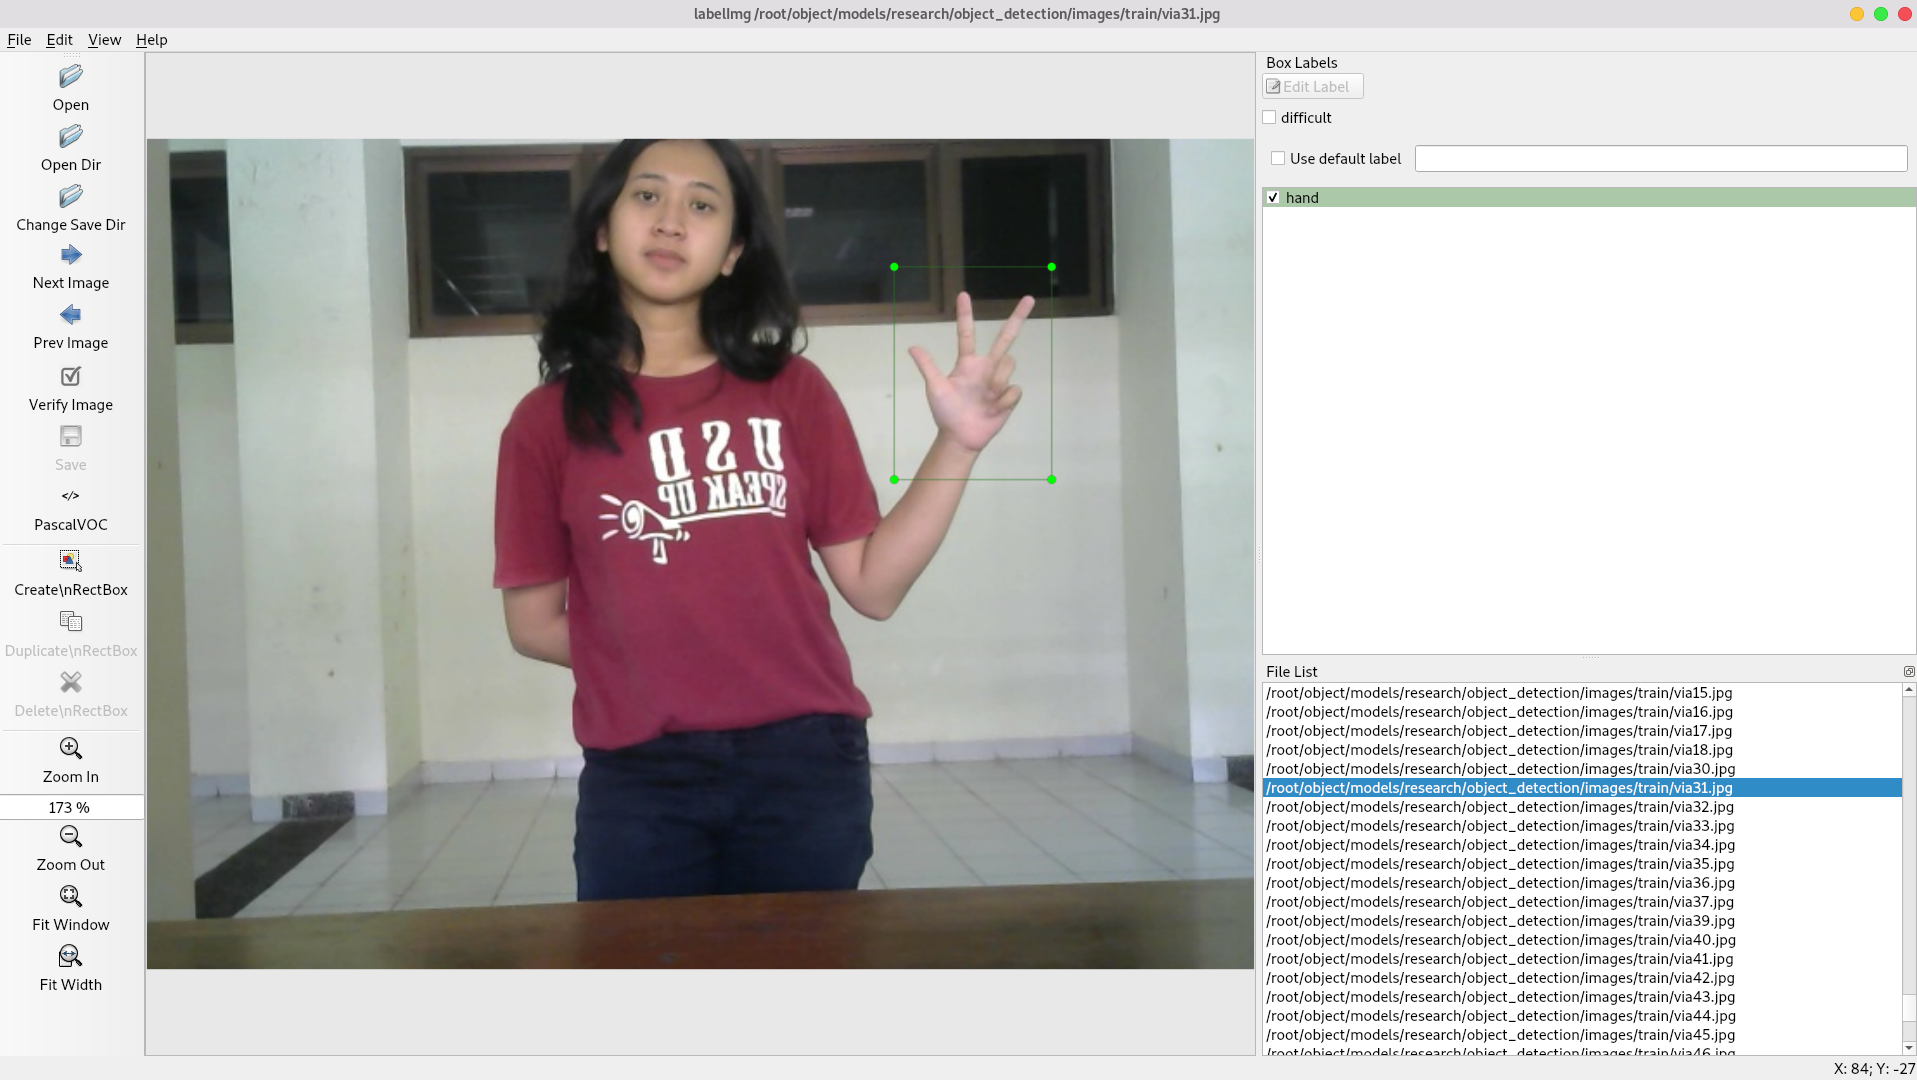
\includegraphics[width=0.8\linewidth]{viany}
	\caption{Proses Pelabelan Citra}
	\label{fig:viany}
\end{figure}
Hasil citra terlabel dijadikan refrensi dalam informasi XML atau anotasi dari citra tertentu. berikut adalah contoh hasil anotasi dari salah satu citra.
% TODO: \usepackage{graphicx} required
\begin{figure}[H]
	\centering
	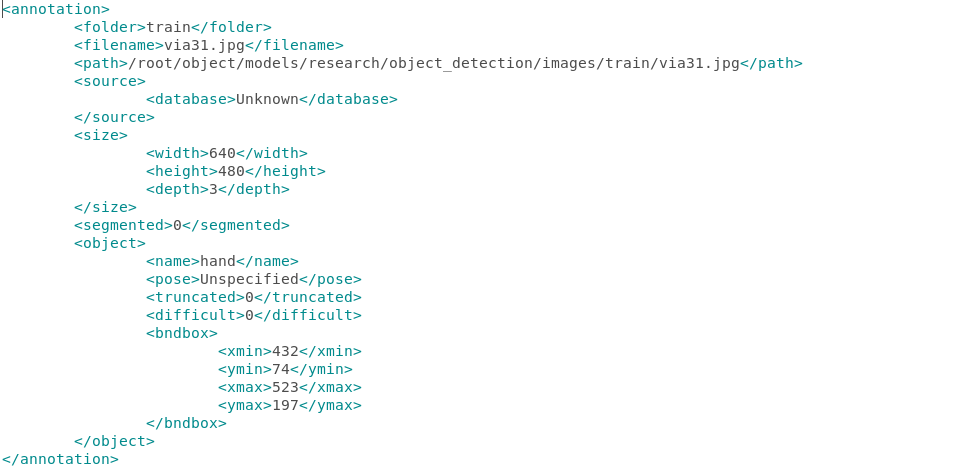
\includegraphics[width=0.8\linewidth]{anotasi}
	\caption{hasil anotasi citra}
	\label{fig:anotasi}
\end{figure}
\section{Implementasi Pembuatan TFRecord file}
Proses selanjutnya adalah mengubah informasi XML ke CSV dengan tujuan membuat format \textit{Tensorflow} dataset atau \textit{TFRecord}. Berikut program konversi file dataset.
\begin{figure}[H]
	\centering
	\lstinputlisting[language=python]{xml.py}
	\caption{Source Code Pengubahan XML ke CSV}
\end{figure}
\begin{figure}[H]
	\centering
	\lstinputlisting[language=python]{tfrecord.py}
	\caption{Source Code Pembentukan TFRecord}
\end{figure}
\section{Konfigurasi \textit{Pipeline Object Detection}}
Proses pelatihan Tensorflow Object Detection API  menggunakan konfigurasi pipeline, beberapa konfigurasi tersebut diantaranya model, training\_config, eval\_config, train\_input\_config, eval\_input\_config. Dataset yang berformat \textit{TFRecord akan di lewatkan sebagai input} dan model pada ssd mobilenet v2 akan digunakan sebagai \textit{pretrained} model. Berikut adalah konfigurasi yang digunakan

\section{Implementasi Training}
\subsection{Object Detection}
Tahap pelatihan dalam \textit{object detection} menggunakan arsitektur mobilenet v2, proses pelatihan berlangsung dengan menggunakan parameter pada konfigurasi pipeline. berikut adalah program untuk melakukan pelatihan.
\begin{figure}[H]
	\centering
	\lstinputlisting[language=python]{training.py}
	\caption{Source Code Pelatihan \textit{Object Detection}}
\end{figure}
\subsection{Pengenalan Gestur}
Pada proses pelatihan gestur menggunakan \textit{k-fold cross validation} dengan k=5. Arsitektur yang digunakan adalah mobilenet v2, pada pelatihan ini \textit{pretrained} model akan di \textit{load} menjadi base model dan jumlah \textit{classifier} diganti sesuai dengan objek yang akan di klasifikasikan dan menambahkan \textit{hidden layer}. Proses tersebut ditunjukan pada program berikut.
\begin{figure}[H]
	\centering
	\lstinputlisting[language=python]{load_pretrained.py}
	\caption{Source Code Pelatihan \textit{Pengenalan Gestur}}
\end{figure}

\section{Implementasi Testing}
Pada implementasi testing dilakukan beberapa pengujian model SNR dan mAP 